\chapter{État de l'art des attaques sur SSL/TLS}

\section{Historique des attaques sur SSL/TLS et HTTPS}

\begin{figure}[H]
  \caption{Historique des attaques SSL/TLS (source : Cloudflare \cite{cloudflare})}
  \fbox{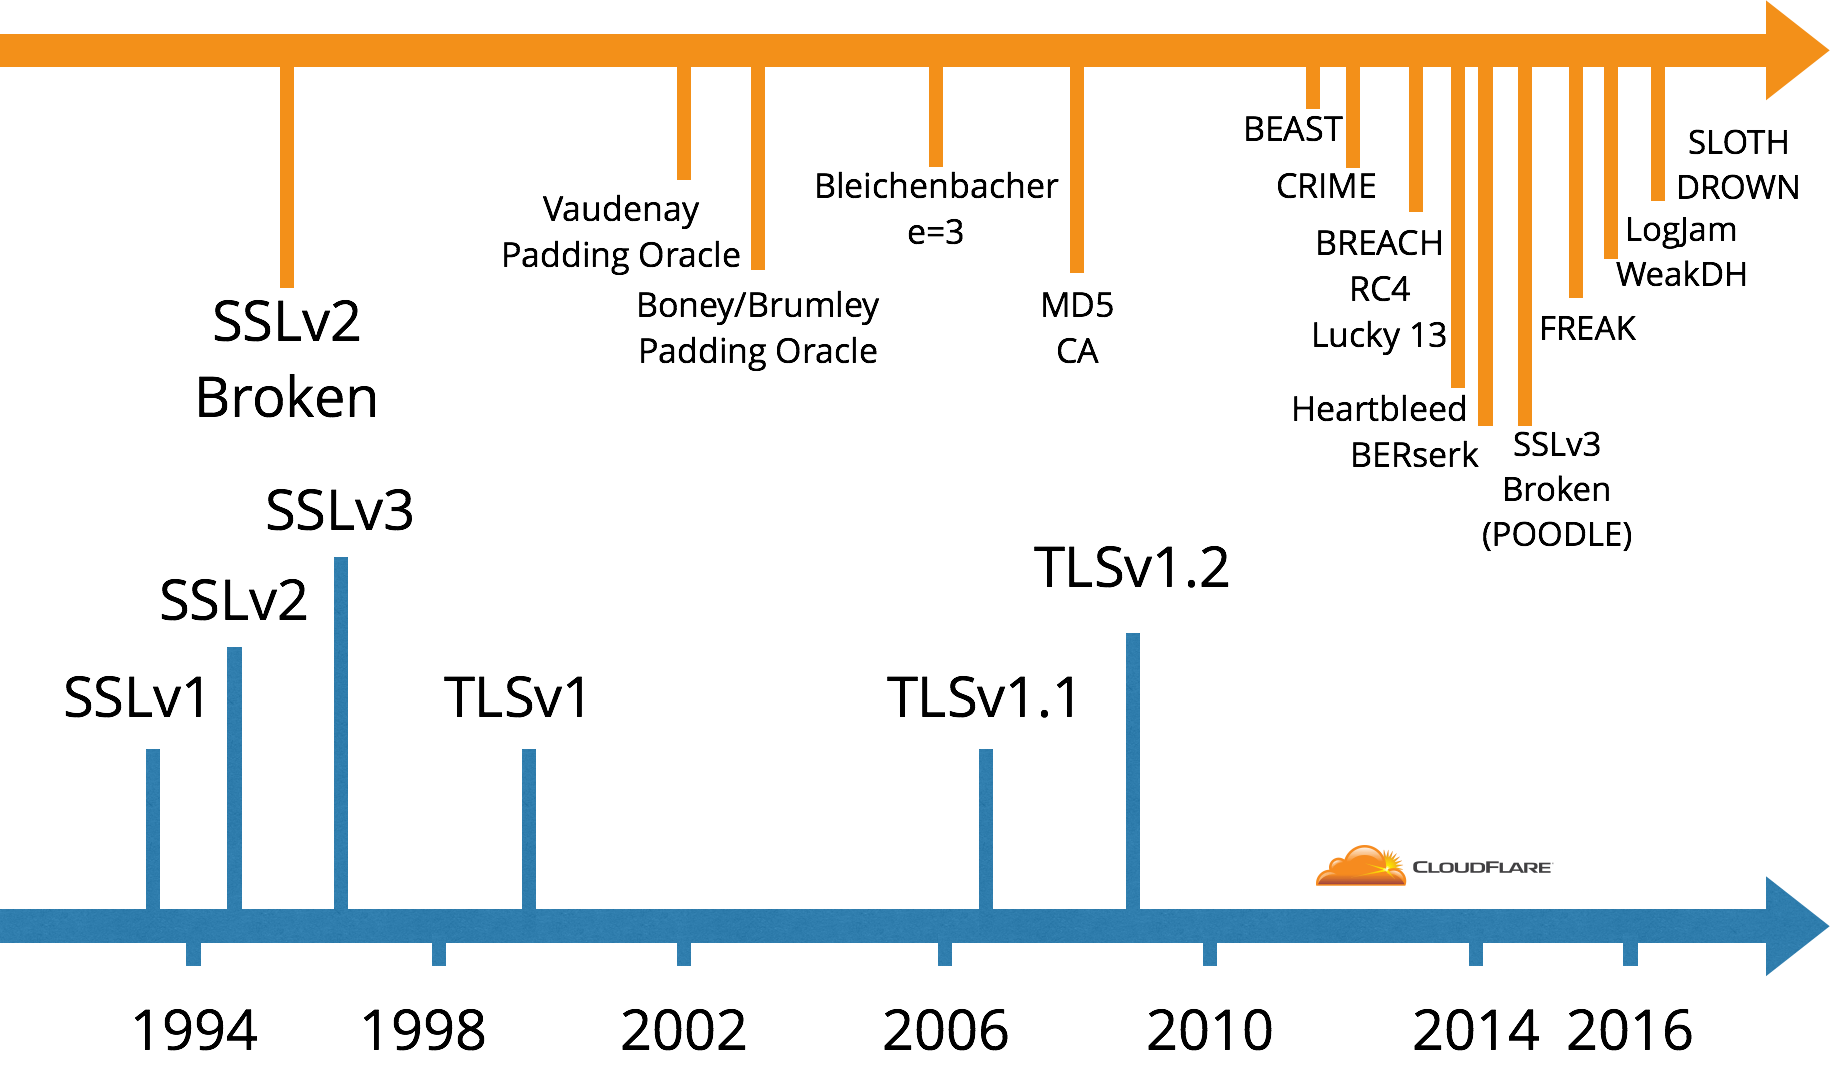
\includegraphics[width=\textwidth]{../medias/history-tls-attacks.png}}
\end{figure}

%%%%%%%%%%%%%%%%%%%%%%%%%%%%%%%%%%%%%%%%%%%%%%%%%%%%%%%%%%%%%%%%%%%%%%%%%%%%%%%%%%
%%%%%%%%%%%%%%%%%%%%%%%%%%%%%%%%%%%%%%%%%%%%%%%%%%%%%%%%%%%%%%%%%%%%%%%%%%%%%%%%%%


\subsection{Interception HTTPS}

\begin{tabularx}{0.96\textwidth}{|c|X|}
  \hline
  \textbf{CVE(s)} & \textbf{Catégorie} \\
  \hline
  - & protocole \\
  \hline
\end{tabularx}

\vspace{1em}

L'interception et le déchiffrement des flux HTTPS (et plus généralement SSL/TLS), est un problème inhérent au fonctionnement du protocole et des CA (certificat authorities).

Un équipement positionné en homme du milieu sur le réseau a la possibilité de fonctionner à la manière d'un proxy : les connexions initiées par les clients pourront être déchiffrées par le proxy, puis rechiffrées vers le serveur. Pour être réalisé de manière transparente, l'idée est de présenter un faux certificat (qui pourra être généré à la volée) au client, qui si il est accepté, permettra le déchiffrement complet des communications entre lui et le serveur.

Pour que ce faux certificat soit accepté, il faut bien sûr que les noms de domaines entre le site visité et le certificat concordent, et que celui-ci soit signé par une autorité de certification connue du client. La manière la plus simple étant d'auto-signer le certificat, en ajoutant sa clef publique dans le navigateur du client. Nous avons également vu par le passé que les autorités de certifications ne sont pas à l'abri d'attaques informatiques, et que de faux certificats légitimes peuvent être émis (on se souviendra par exemple de DigiNotar en 2011) \cite{https-interception}.

Cette attaque est détaillée dans le chapitre \hyperref[sec:https-interception]{Interception HTTPS}.

%%%%%%%%%%%%%%%%%%%%%%%%%%%%%%%%%%%%%%%%%%%%%%%%%%%%%%%%%%%%%%%%%%%%%%%%%%%%%%%%%%
%%%%%%%%%%%%%%%%%%%%%%%%%%%%%%%%%%%%%%%%%%%%%%%%%%%%%%%%%%%%%%%%%%%%%%%%%%%%%%%%%%


\subsection{SSLsniff (2002)}

\begin{tabularx}{0.96\textwidth}{|c|X|}
  \hline
  \textbf{CVE(s)} & \textbf{Catégorie} \\
  \hline
  CAN-2002-0862 & implémentation, certificats \\
  \hline
\end{tabularx}

\vspace{1em}

SSLsniff est une attaque ciblant le navigateur Internet Explorer de Microsoft. La validation d'un certificat par ce navigateur n'était pas réalisée de manière adéquate. Un certificat feuille signé par une autorité de certification légitime pouvait alors signer un certificat pour n'importe quel domaine, et être accepté par le navigateur. Ceci était possible, car le navigateur ne vérifiait pas le champ ``Basic Constraints'' du certificat, précisant si le certificat est une CA ou non. L'outil SSLsniff permet l'automatisation de cette attaque \cite{sslsniff-website}.


%%%%%%%%%%%%%%%%%%%%%%%%%%%%%%%%%%%%%%%%%%%%%%%%%%%%%%%%%%%%%%%%%%%%%%%%%%%%%%%%%%
%%%%%%%%%%%%%%%%%%%%%%%%%%%%%%%%%%%%%%%%%%%%%%%%%%%%%%%%%%%%%%%%%%%%%%%%%%%%%%%%%%


\subsection{SSLstrip (2009)}

\begin{tabularx}{0.96\textwidth}{|c|X|}
  \hline
  \textbf{CVE(s)} & \textbf{Catégorie} \\
  \hline
  - & protocole, humain \\
  \hline
\end{tabularx}

\vspace{1em}

L'attaque SSLstrip ne vise pas les connexion HTTPS chiffrées et authentifiées, mais plutôt les connexions HTTP falsifiables facilement. Un attaquant situé en homme du milieu peut modifier les réponses d'un serveur, afin de remplacer tous les liens sécurisés (https://) par leur version non-sécurisée (http://) en prenant également en compte les éventuelles redirections (code HTTP 302).

Le client, si il n'est pas attentif, utilisera alors des connections HTTP non sécurisée lors de sa navigation à la place d'une connexion HTTPS. Afin de rester transparent pour le serveur, l'attaquant peut alors rediriger les requêtes HTTP du client, vers leurs équivalent HTTPS vers le serveur \cite{sslstrip-website}.

Cette attaque est détaillée dans le chapitre \hyperref[sec:sslstrip]{SSLstrip}.

%%%%%%%%%%%%%%%%%%%%%%%%%%%%%%%%%%%%%%%%%%%%%%%%%%%%%%%%%%%%%%%%%%%%%%%%%%%%%%%%%%
%%%%%%%%%%%%%%%%%%%%%%%%%%%%%%%%%%%%%%%%%%%%%%%%%%%%%%%%%%%%%%%%%%%%%%%%%%%%%%%%%%


\subsection{BEAST (2011)}

\begin{tabularx}{0.96\textwidth}{|c|X|}
  \hline
  \textbf{CVE(s)} & \textbf{Catégorie} \\
  \hline
  CVE-2011-3389 & cryptographie \\
  \hline
\end{tabularx}

\vspace{1em}

L'attaque BEAST (Browser Exploit Against SSL/TLS) concerne SSL 3.0 et TLS 1.0. L'attaquant, placé en Man-in-the-Middle, peut déchiffrer les données échangées entre le serveur et le client grâce à une vulnérabilité d'implémentation du mode CBC, Cipher Block Chaining. L'attaque se fait côté client en injectant des paquets dans le flux TLS. Cette technique est qualifiée d'attaque à clair connu. La faille du protocole réside dans le chiffrement par bloc. En effet, les blocs sont chiffrés les uns après les autres en utilisant le précédent \cite{beast}.

Voici le déroulement de l'attaque :

\begin{enumerate}
\item Injection du code chez la victime
\item La victime envoie des données forgées via SSL
\item L'attaquant écoute le trafic
\item Il renvoie les informations nécessaires à son code injecté
\item La victime renvoie les données forgées et on répète les deux étapes précédentes
  \item L'attaquant dérive tous les cookies
\end{enumerate}

%%%%%%%%%%%%%%%%%%%%%%%%%%%%%%%%%%%%%%%%%%%%%%%%%%%%%%%%%%%%%%%%%%%%%%%%%%%%%%%%%%
%%%%%%%%%%%%%%%%%%%%%%%%%%%%%%%%%%%%%%%%%%%%%%%%%%%%%%%%%%%%%%%%%%%%%%%%%%%%%%%%%%


\subsection{CRIME (2012)}

\begin{tabularx}{0.96\textwidth}{|c|X|}
  \hline
  \textbf{CVE(s)} & \textbf{Catégorie} \\
  \hline
  CVE-2012-4929 & cryptographie, protocole \\
  \hline
\end{tabularx}

\vspace{1em}

CRIME (compression ratio info-leak made easy), utilise une faille de l'algorithme de compression utilisé par TLS. Cette attaque vise surtout les cookies de sessions. L'idée est d'envoyer des caractères aléatoires dans un cookie forgé et de comparer la compression de ce dernier avec le cookie originel du client. Si le cookie forgé est partiellement compressé, on peut inférer qu'une partie de ce dernier correspondant au cookie du client. On procède ainsi par étapes successives pour retrouver le cookie et voler la session de la victime.

Cette attaque nécessite que l'attaquant se place en MITM pour pouvoir observer la taille du chiffré envoyé par le client mais également pouvoir envoyer des requêtes forgées par l'attaquant lui-même \cite{crime}.


%%%%%%%%%%%%%%%%%%%%%%%%%%%%%%%%%%%%%%%%%%%%%%%%%%%%%%%%%%%%%%%%%%%%%%%%%%%%%%%%%%
%%%%%%%%%%%%%%%%%%%%%%%%%%%%%%%%%%%%%%%%%%%%%%%%%%%%%%%%%%%%%%%%%%%%%%%%%%%%%%%%%%


\subsection{BREACH (2012)}

\begin{tabularx}{0.96\textwidth}{|c|X|}
  \hline
  \textbf{CVE(s)} & \textbf{Catégorie} \\
  \hline
  - & cryptographie, protocole \\
  \hline
\end{tabularx}

\vspace{1em}


L'attaque BREACH (Browser reconnaissance and exfiltration via adaptive compression of hypertext) est en grande partie similaire à CRIME vue plus haut. Cette fois ci ce n'est pas la compression TLS mais plutôt celle effectuée par HTTP qui est visée \cite{breach}.


%%%%%%%%%%%%%%%%%%%%%%%%%%%%%%%%%%%%%%%%%%%%%%%%%%%%%%%%%%%%%%%%%%%%%%%%%%%%%%%%%%
%%%%%%%%%%%%%%%%%%%%%%%%%%%%%%%%%%%%%%%%%%%%%%%%%%%%%%%%%%%%%%%%%%%%%%%%%%%%%%%%%%


\subsection{Cassage de RC4 (2013)}

\begin{tabularx}{0.96\textwidth}{|c|X|}
  \hline
  \textbf{CVE(s)} & \textbf{Catégorie} \\
  \hline
  CVE-2013-2566 & cryptographie \\
  \hline
\end{tabularx}

\vspace{1em}


RC4 est un algorithme de chiffrement symétrique par flots qui était majoritairement utilisé pour protéger le trafic TLS.

La première attaque mise en place pour casser l'algorithme RC4 se base sur une attaque multi-session. C'est-à-dire que l'on a besoin d'envoyer un message clair cible à plusieurs reprises positionné au même endroit dans le flux TLS. L'exploitation se fait grâce à un biais d'un des octets du keystream en se focalisant sur les 100 premiers octets de celui-ci. Les 36 premiers octets de l'échange TLS chiffré étant un message de type ``Finished Message'' imprévisible, il est impossible d'attaquer ces octets du keystream : il sera alors possible de déchiffrer environ 64 octets du message chiffré. Le nombre de connexions nécessaires pour l'attaque peut être variable. L'attaquant peut mettre fin à la session TLS et certaines applications s'exécutant sur TLS se reconnectent automatiquement et retransmettent un cookie ou un mot de passe. Dans un environnement web, les sessions peuvent aussi être générées par du code malveillant côté client à travers du JavaScript, comme pour l'attaque BEAST.

La deuxième attaque s'applique à TLS et peut être effectuée grâce à une seule connexion. On exploite certains double octets dans le flux de clés RC4. On cible les octets en clair situés à n'importe quelle position dans le flux de texte clair TLS. Le nombre de messages chiffrés nécessaire pour récupérer de façon fiable un ensemble de 16 octets de textes clair ciblés consécutifs est d'environ $10*2^{30}$, mais avec seulement $6*2^{30}$, ces octets peuvent être récupérés avec une fiabilité de 50\%. Cette attaque peut être plus efficace en pratique.

Dans cette attaque, l'attaquant peut se trouver dans n'importe où sur le chemin réseau entre le client et le serveur\cite{rc4}.


%%%%%%%%%%%%%%%%%%%%%%%%%%%%%%%%%%%%%%%%%%%%%%%%%%%%%%%%%%%%%%%%%%%%%%%%%%%%%%%%%%
%%%%%%%%%%%%%%%%%%%%%%%%%%%%%%%%%%%%%%%%%%%%%%%%%%%%%%%%%%%%%%%%%%%%%%%%%%%%%%%%%%


\subsection{Lucky13 (2013)}

\begin{tabularx}{0.96\textwidth}{|c|X|}
  \hline
  \textbf{CVE(s)} & \textbf{Catégorie} \\
  \hline
  CVE-2013-0169 & implémentation, cryptographie, canaux auxiliaires \\
  \hline
\end{tabularx}

\vspace{1em}

Lucky 13 fait encore partie du cadre d'attaque MITM. La faille permet à un attaquant de récupérer du texte clair à partir d'une connexion TLS lorsque que le cryptage en mode CBC est utilisé. Comme l'attaque précédente, on effectue des attaques à plusieurs sessions, donc on a besoin d'envoyer un message clair cible à plusieurs reprise dans la même position dans le flux de texte lors de plusieurs connexions TLS. On détecte de petites différences dans l'heure à laquelle les messages d'erreur TLS apparaissent sur le réseau en réponse à des textes chiffrés générés par l'attaquant. L'attaquant doit récupérer plusieurs échantillons pour une même heure car il y a souvent des perturbations \cite{lucky13}.

Le nombre de session nécessaire est donc :

\begin{itemize}
\item 223 si l'attaquant se trouve sur le même LAN que la machine attaquée et que HMAC-SHA1 est utilisé comme algorithme MAC (Message Authentication Code) de TLS.
\item 219 si le texte clair est codé en base64.
\item 213 si un octet du texte clair dans l'une des deux dernières positions d'un bloc est déjà connu.
\end{itemize}


%%%%%%%%%%%%%%%%%%%%%%%%%%%%%%%%%%%%%%%%%%%%%%%%%%%%%%%%%%%%%%%%%%%%%%%%%%%%%%%%%%
%%%%%%%%%%%%%%%%%%%%%%%%%%%%%%%%%%%%%%%%%%%%%%%%%%%%%%%%%%%%%%%%%%%%%%%%%%%%%%%%%%


\subsection{Heartbleed (2014)}

\begin{tabularx}{0.96\textwidth}{|c|X|}
  \hline
  \textbf{CVE(s)} & \textbf{Catégorie} \\
  \hline
  CVE-2014-0160 & implémentation \\
  \hline
\end{tabularx}

\vspace{1em}

Il s'agit d'une vulnérabilité présente dans la bibliothèque cryptographique OpenSSL, notamment dans l'extension Heartbeat de SSL/TLS (RFC 6520). Ce protocole permet de maintenir la connexion active (à la manière d'un ping), et une erreur de programmation dans la bibliothèque permettait de provoquer une fuite de la mémoire d'un serveur impacté. Dans ce cas, le client peut envoyer un paquet Heartbeat avec un champ ``longueur'' excédant la longueur réelle du paquet. En réponse à ce dernier, le serveur vulnérable répond avec un paquet contenant une partie de sa mémoire.

Il est alors possible de récupérer à travers cette vulnérabilité un certain nombre d'informations confidentielles : clefs de sessions, clefs privées, cookies de sessions, mots de passe utilisateurs...\cite{heartbleed}.


%%%%%%%%%%%%%%%%%%%%%%%%%%%%%%%%%%%%%%%%%%%%%%%%%%%%%%%%%%%%%%%%%%%%%%%%%%%%%%%%%%
%%%%%%%%%%%%%%%%%%%%%%%%%%%%%%%%%%%%%%%%%%%%%%%%%%%%%%%%%%%%%%%%%%%%%%%%%%%%%%%%%%


\subsection{BERserk (2014)}

\begin{tabularx}{0.96\textwidth}{|c|X|}
  \hline
  \textbf{CVE(s)} & \textbf{Catégorie} \\
  \hline
  CVE-2014-1569 & implémentation, cryptographie \\
  \hline
\end{tabularx}

\vspace{1em}

Cette vulnérabilité concerne la bibliothèque Mozilla Network Security Services (NSS) utilisée notamment dans les logiciels Mozilla. L'attaque repose sur la falsification de signature numérique. La faille est présente à cause de l'analyse incorrecte de messages codés en ASN.1 lors de la vérification de signatures RSA.

Les messages ASN.1 sont constitués de diverses parties codées à l'aide de BER (Basic Encoding Rule) et DER (Distinguished Encoding Rules). C'est une variation de l'attaque de Bleichenbacher sur le padding PKCS\#1. Cette attaque exploite le fait que la longueur d'un champ dans le codage BER peut être utilisée pour utiliser de nombreux octets de données. Dans les implémentations vulnérables, ces octets sont ensuite ignorés lors de l'analyse.

Un attaquant peut donc se créer sa clé et se placer dans une situation de man-in-the-middle. Dans ce cas, il intercepte les communications qui seront en clair pour lui car il aura chiffré celle-ci avec sa clé. Pour l'utilisateur, la connexion reste sécurisée et en plus, il verra toujours du HTTPS \cite{berserk}.


%%%%%%%%%%%%%%%%%%%%%%%%%%%%%%%%%%%%%%%%%%%%%%%%%%%%%%%%%%%%%%%%%%%%%%%%%%%%%%%%%%
%%%%%%%%%%%%%%%%%%%%%%%%%%%%%%%%%%%%%%%%%%%%%%%%%%%%%%%%%%%%%%%%%%%%%%%%%%%%%%%%%%


\subsection{POODLE (2014)}

\begin{tabularx}{0.96\textwidth}{|c|X|}
  \hline
  \textbf{CVE(s)} & \textbf{Catégorie} \\
  \hline
  CVE-2014-3566 & cryptographie, protocole \\
  \hline
\end{tabularx}

\vspace{1em}

L'anagramme POODLE signifie "padding oracle on downgraded legacy encryption". L'attaque concerne surtout le protocole SSLv3, bien qu'une variante de la faille fut trouver sur TLS peu de temps après.

Lorsque le message à envoyer est trop court pour l'algorithme de chiffrement par bloc sous-jacent, on lui rajoute un ``padding'' afin de pouvoir appliquer l'algorithme sur le message.

Bien que le TLS soit un protocole plus sûr que SSL et recommandé aujourd'hui, de nombreux serveurs continuent d'accepter le SSL 3.0 si une connexion par TLS venait à être impossible. L'attaque POODLE se sert de ce fait pour forcer la connexion à se faire en SSL.

La vulnérabilité en elle-même vient de la façon dont sont encodés les blocs de donnés avec SSL. L'attaquant a besoin de deux choses pour se faire :

\begin{enumerate}
    \item L'attaquant doit pouvoir changer une partie du message injecté par le client dans l'algorithme
    \item Il doit avoir un retour sur le texte chiffré par SSL.
\end{enumerate}

Ces deux conditions peuvent s'exécuter avec par exemple une attaque en homme du milieu. L'attaquant doit toutefois avoir un contrôle également sur le client pour modifier le padding, ce qui est une tâche supplémentaire à effectuer.

En modifiant le padding, l'attaque permet de récupérer un byte d'information du message initial en envoyant un maximum de 256 requêtes. Cela peut amener l'attaquant à envoyer énormément de requêtes pour obtenir le message dans son intégralité.

L'avantage de cette attaque est qu'elle ne nécessite pas de connaître la clef utilisée pour le chiffrement \cite{poodle}.


%%%%%%%%%%%%%%%%%%%%%%%%%%%%%%%%%%%%%%%%%%%%%%%%%%%%%%%%%%%%%%%%%%%%%%%%%%%%%%%%%%
%%%%%%%%%%%%%%%%%%%%%%%%%%%%%%%%%%%%%%%%%%%%%%%%%%%%%%%%%%%%%%%%%%%%%%%%%%%%%%%%%%

\subsection{Attaque SSLstrip2 ou SSLstrip+ (2014)}

\begin{tabularx}{0.96\textwidth}{|c|X|}
  \hline
  \textbf{CVE(s)} & \textbf{Catégorie} \\
  \hline
  - & protocole, humain \\
  \hline
\end{tabularx}

\vspace{1em}

Cette nouvelle version de SSLstrip permet de contourner une sécurité ajoutée à TLS : le HSTS (voir section \hyperref[sec:hsts]{Contremesures - HSTS}).

Avec cette protection, on ne va donc plus pouvoir simplement strippé le 's' de HTTPS pour inciter le client à envoyer sa requête en HTTP (et ainsi permettre à l'attaquer de voir tout le trafic en clair). Le navigateur émettra en effet une exception car il aura gardé en mémoire dans une base de donnée qu'il doit toujours se connecter en HTTPS sur le serveur en question.

Pour cette attaque, l'attaquant doit se situer en man in the middle. Lorsque le client va se connecter au serveur sur une page en HTTP, l'attaquant va intercepter la réponse du serveur, et modifier sur cette page les liens qui renvoient vers du HTTPS. Si le lien est par exemple https://www.domain.secure, on va le remplacer par http://wwww.domain.secure. On peut enlever le 's' ici, car le navigateur ne connaît pas ce nom de domaine : il ne l'a encore jamais visité. Il va donc envoyer une requête DNS que l'attaquant va intercepter et remplacer par l'adresse IP réelle du serveur.

Ainsi il va pouvoir faire croire au navigateur du client que tout est légitime, et que wwww.domain.secure correspond bien au serveur distant. Le navigateur n'ayant pas enregistré dans sa base donnée qu'il devait se connecter en HTTPS sur wwww.domain.secure, il va donc accepter d'envoyer sa requête en HTTP, laissant encore une fois tout son trafic au clair aux yeux de l'attaquant !

Cette attaque est détaillée dans le chapitre \hyperref[sec:sslstrip2]{SSLstrip+}.

%%%%%%%%%%%%%%%%%%%%%%%%%%%%%%%%%%%%%%%%%%%%%%%%%%%%%%%%%%%%%%%%%%%%%%%%%%%%%%%%%%
%%%%%%%%%%%%%%%%%%%%%%%%%%%%%%%%%%%%%%%%%%%%%%%%%%%%%%%%%%%%%%%%%%%%%%%%%%%%%%%%%%

\subsection{SSLstrip-NTP (2014}

\begin{tabularx}{0.96\textwidth}{|c|X|}
  \hline
  \textbf{CVE(s)} & \textbf{Catégorie} \\
  \hline
  - & protocole, humain \\
  \hline
\end{tabularx}

\vspace{1em}

Cette amélioration de l'attaque SSLstrip originale a été présentée pour la première fois par Jose Selvi à la Blackhat Europe de 2014. Celle-ci permet de contourner la sécurité offerte par HSTS (HTTP Strict Transport Security), dans le cas où l'attaquant est capable de modifier le trafic NTP entre le client et le serveur NTP.

L'attaque consiste à expirer les entrées HSTS de la machine cliente en modifiant l'horloge ce celle-ci, grâce à l'usurpation des requêtes NTP. Une fois les entrées HSTS expirées, l'attaquant peut utiliser l'attaque SSLstrip originale pour stripper les liens https des pages web visitées par la victime \cite{sslstrip-ntp}.

Cette attaque est détaillée dans le chapitre \hyperref[sec:sslstrip-ntp]{SSLstrip NTP}.

%%%%%%%%%%%%%%%%%%%%%%%%%%%%%%%%%%%%%%%%%%%%%%%%%%%%%%%%%%%%%%%%%%%%%%%%%%%%%%%%%%
%%%%%%%%%%%%%%%%%%%%%%%%%%%%%%%%%%%%%%%%%%%%%%%%%%%%%%%%%%%%%%%%%%%%%%%%%%%%%%%%%%

\subsection{FREAK (2015)}

\begin{tabularx}{0.96\textwidth}{|c|X|}
  \hline
  \textbf{CVE(s)} & \textbf{Catégorie} \\
  \hline
  CVE-2015-0204 & cryptographie, protocole \\
  \hline
\end{tabularx}

\vspace{1em}

FREAK (factorising RSA export keys) a pour origine l'exportation de la cryptographie des USA qui gardait pour eux les meilleurs systèmes et partageait les moins bons avec le reste du monde, afin que la NSA puisse les craquer avec leur puissance de calcul supérieur.

Vers 2010, avec la montée en puissance constante des ordinateurs, tout le monde est maintenant capable avec un "bon pc" de craquer ces clés plus faibles, les "export-keys".

Le but de l'attaque est donc de forcer la connexion client/serveur de la victime a utiliser ces clefs plus faibles au lieu des clefs RSA standards plus fortes utilisées aujourd'hui \cite{freak}.


%%%%%%%%%%%%%%%%%%%%%%%%%%%%%%%%%%%%%%%%%%%%%%%%%%%%%%%%%%%%%%%%%%%%%%%%%%%%%%%%%%
%%%%%%%%%%%%%%%%%%%%%%%%%%%%%%%%%%%%%%%%%%%%%%%%%%%%%%%%%%%%%%%%%%%%%%%%%%%%%%%%%%


\subsection{WeakDH (2015)}

\begin{tabularx}{0.96\textwidth}{|c|X|}
  \hline
  \textbf{CVE(s)} & \textbf{Catégorie} \\
  \hline
  - & cryptographie \\
  \hline
\end{tabularx}

\vspace{1em}

La vulnérabilité WeakDH concerne les paramètres du protocole Diffie-Hellman utilisés dans certaines implémentations, en particulier le corps $\mathbb{Z}/p\mathbb{Z}$ choisi. En effet, le nombre premier utilisé par celles-ci (environ 8.4\% du top million Alexa lors de la découverte de WeakDH)), est d'une part relativement petit (1024 bits) ce qui le rend vulnérable à la recherche du logarithme discret en un temps raisonnable, et d'autre part, puisque le même nombre premier était utilisé, les efforts pour attaquer un site était le même que pour attaquer l'ensemble des sites utilisant ce nombre premier\cite{weakdh}.


%%%%%%%%%%%%%%%%%%%%%%%%%%%%%%%%%%%%%%%%%%%%%%%%%%%%%%%%%%%%%%%%%%%%%%%%%%%%%%%%%%
%%%%%%%%%%%%%%%%%%%%%%%%%%%%%%%%%%%%%%%%%%%%%%%%%%%%%%%%%%%%%%%%%%%%%%%%%%%%%%%%%%


\subsection{Logjam (2015)}

\begin{tabularx}{0.96\textwidth}{|c|X|}
  \hline
  \textbf{CVE(s)} & \textbf{Catégorie} \\
  \hline
  CVE-2015-4000 & cryptographie, protocole \\
  \hline
\end{tabularx}

\vspace{1em}

Logjam concerne l'algorithme Diffie-Hellman qui est mis en place lors du protocole TLS au moment de de la poignée de main initiale. Cette dernière étant un algorithme permettant d'échanger les clés et négocier la connexion sécurisée. L'attaquant, placé en MITM, peut écouter toutes connexions TLS qui utilisent de la cryptographie basée sur 512 bits. L'attaque affecte les serveurs qui prennent en charge les chiffrements DHE\_EXPORT. Ce chiffrement requiert un nombre premier court de 512 bits. Précisons que cette faiblesse a été créée volontairement pour satisfaire une réglementation des années 90
\cite{logjam}.


%%%%%%%%%%%%%%%%%%%%%%%%%%%%%%%%%%%%%%%%%%%%%%%%%%%%%%%%%%%%%%%%%%%%%%%%%%%%%%%%%%
%%%%%%%%%%%%%%%%%%%%%%%%%%%%%%%%%%%%%%%%%%%%%%%%%%%%%%%%%%%%%%%%%%%%%%%%%%%%%%%%%%


\subsection{DROWN (2016)}

\begin{tabularx}{0.96\textwidth}{|c|X|}
  \hline
  \textbf{CVE(s)} & \textbf{Catégorie} \\
  \hline
  CVE-2016-0800 & cryptographie, protocole \\
  \hline
\end{tabularx}

\vspace{1em}

Drown (Decrypting RSA with Obsolete and Weakened eNcryption) affecte HTTPS, SSL et TLS. Lors de la découverte de cette attaque, les serveurs utilisaient majoritairement TLS, néanmoins, ils supportaient aussi SSLv2. Cette prise en charge a constitué une menace, car l'attaquant peut déchiffrer des connexions TLS en envoyant des sondes à un serveur qui prend en charge SSLv2 et utilise la même clé. L'exploitation de cette faille passe par une attaque à chiffré choisi \cite{drown}.


%%%%%%%%%%%%%%%%%%%%%%%%%%%%%%%%%%%%%%%%%%%%%%%%%%%%%%%%%%%%%%%%%%%%%%%%%%%%%%%%%%
%%%%%%%%%%%%%%%%%%%%%%%%%%%%%%%%%%%%%%%%%%%%%%%%%%%%%%%%%%%%%%%%%%%%%%%%%%%%%%%%%%


\subsection{SLOTH (2016)}

\begin{tabularx}{0.96\textwidth}{|c|X|}
  \hline
  \textbf{CVE(s)} & \textbf{Catégorie} \\
  \hline
  CVE-2015-7575 & cryptographie, protocole \\
  \hline
\end{tabularx}

\vspace{1em}

Sloth (Security Losses from Obsolete and Truncated Transcript Hashes) s'intéresse à la perte de sécurité due à l'utilisation d'algorithmes de hachage obsolètes au sein des protocoles cryptographiques. Les algorithmes particulièrement ciblés sont SHA-1 et MD5 utilisés à cette époque dans TLS 1.1, TLS 1.2 et TLS 1.3 . Sloth est basée sur une attaque par collision par transposition et permet de réduire la sécurité de 128 bits à 64 bits \cite{sloth}.


%%%%%%%%%%%%%%%%%%%%%%%%%%%%%%%%%%%%%%%%%%%%%%%%%%%%%%%%%%%%%%%%%%%%%%%%%%%%%%%%%%
%%%%%%%%%%%%%%%%%%%%%%%%%%%%%%%%%%%%%%%%%%%%%%%%%%%%%%%%%%%%%%%%%%%%%%%%%%%%%%%%%%


\subsection{SWEET32 (2016)}

\begin{tabularx}{0.96\textwidth}{|c|X|}
  \hline
  \textbf{CVE(s)} & \textbf{Catégorie} \\
  \hline
  CVE-2016-2183 & cryptographie \\
  \hline
\end{tabularx}

\vspace{1em}

Sweet32 est une attaque qui vise les algorithmes symétriques utilisant des blocs inférieurs ou égaux à 64 bits utilisant le mode CBC. Il faut utiliser encore une fois une attaque par collision basée sur le paradoxe des anniversaires. En collectant environ 32Go de données chiffrées, l'attaquant a alors une grande probabilité de trouver deux blocs chiffrés identiques. En ayant une connaissance d'une partie du texte en clair il a la possibilité de déchiffrer certains blocs. Cette attaque a particulièrement affaibli les algorithmes 3-DES et blowfish, tous deux opérant sur des blocs de 64bits \cite{sweet32}.


%%%%%%%%%%%%%%%%%%%%%%%%%%%%%%%%%%%%%%%%%%%%%%%%%%%%%%%%%%%%%%%%%%%%%%%%%%%%%%%%%%
%%%%%%%%%%%%%%%%%%%%%%%%%%%%%%%%%%%%%%%%%%%%%%%%%%%%%%%%%%%%%%%%%%%%%%%%%%%%%%%%%%


\subsection{ROBOT (2017)}

\begin{tabularx}{0.96\textwidth}{|c|X|}
  \hline
  \textbf{CVE(s)} & \textbf{Catégorie} \\
  \hline
  CVE-2017-13099 & cryptographie, implémentation \\
  \hline
\end{tabularx}

\vspace{1em}

La vulnérabilité ROBOT (Return Of the Bleichenbacher's Oracle Threat), est une attaque sur le padding RSA PKCS\#1 v1.5 de certaines implémentations de SSL/TLS (F5, Citrix, Radware, Cisco, Erlang, Bouncy Castle et WolfSSL). Celle-ci permet de déchiffrer l'intégralité des messages chiffrés avec l'algorithme RSA ou de forger des signatures grâce à un oracle de padding et les travaux de Bleichenbacher\cite{robot}.


\section{Contremesures et protections}

\subsection{HSTS}

\label{sec:hsts}

HTTP Strict Transport Security (HSTS) est un mécanisme de sécurité décrit dans la RFC6797 permettant à un serveur HTTP de déclarer à ses clients que ces derniers doivent toujours utiliser une communication sécurisée en HTTPS pour leurs futures communications avec lui. Pour cela, le serveur envoit l'entête ``Strict-Transport-Security'', en précisant la durée pendant laquelle le client devra utiliser une connexion sécurisée \cite{hsts}.

Ce mécanisme a été mis en place notamment pour contrer l'attaque SSLstrip initiale. Bien entendu, cette contremesure ne protège pas la première connexion initiée par le client. Pour protéger la première connexion, les navigateurs récents ont mis en place une liste pré-chargée des domaines utilisant HSTS. Par exemple, il est possible d'enregistrer un domaine pour le navigateur Chrome sur le site \url{https://hstspreload.org/} pour faire figurer le domaine dans cette liste.

Lorsque le navigateur a enregistré un nom de domaine protégé par HSTS, celui-ci remplacera tous les liens http:// par leurs équivalent https:// pour le domaine (ou sous-domaine) concerné. De plus, si le certificat est invalide (auto-signé par exemple), le navigateur affichera un message d'erreur et empêchera l'utilisateur de se connecter au site.

Pour firefox par exemple, cette base de donnée est stockée dans le fichier \path{SiteSecurityServiceState.txt} présent dans le profile Mozilla firefox.

Voici par à quoi correspond une entrée de ce fichier, ici pour le domaine www.youtube.com :

\begin{minted}[bgcolor=lbcolor, breaklines]{text}
www.youtube.com:HSTS    24      17594   155170223888,1,0,2
\end{minted}

Les deux premiers nombres correspondent à la fréquence de visites du domaine, le troisième (155170223888) est le nombre de millisecondes avant expiration de l'entrée, le quatrième (1) est l'état de l'entrée, ici active. Le cinquième (0) spécifie si il faut appliquer HSTS aux sous-domaines (ici, non), et le dernier chiffre (2) indique la source de l'entrée (Unknown, Preload, Organic). Ici donc Organic, c'est à dire récupérée grâce à l'entête HTTP.

\subsection{HPKP}

HTTP Public Key Pinning est un autre mécanisme de sécurité décrit dans la RFC7469, qui permet à un serveur de transmettre à ses clients les empreintes de ses certificats, via un entête HTTP. Un client supportant ce mécanisme stockera alors cette empreinte pour une certaine durée (précisée par le serveur). Si l'empreinte du certificat a changé, le client refusera alors de se connecter au serveur \cite{hpkp}.

Ceci permet en particulier de se protéger de l'interception HTTPS réalisée avec un certificat frauduleux. Comme HSTS, ce mécanisme ne protège pas la première connexion, mais seulement les futures conxexions.

Pour firefox par exemple, cette correspondance domaine/empreinte est stockée également dans le fichier \path{SiteSecurityServiceState.txt}, présent dans le profile de Mozilla firefox.

Voici à quoi ressemble une entrée dans ce fichier pour HPKP :

\begin{minted}[bgcolor=lbcolor, breaklines]{text}
  services.addons.mozilla.org:HPKP        22      17593   1525287814584,1,1,
  WoiWRyIOVNa9ihaBciRSC7XHjliYS9VwUGOIud4PB18=
  r/mIkG3eEpVdm+u/ko/cwxzOMo1bk4TyHIlByibiA5E=
\end{minted}

Nous voyons l'empreinte du certificat encodé en base64, le nombre de millisecondes avant expiration, que l'entrée est active et que cette empreinte s'applique également aux sous-domaines.

\subsection{DANE/TLSA}

Le mécanisme DANE/TLSA décrit dans la RFC-6698 permet d'enregistrer dans la zone DNS d'un domaine, les empreintes cryptographiques des certificats utilisés par ce domaine. Avec l'utilisation de DNSSEC (protocole permettant de signer les requêtes DNS), ceci permet de vérifier à travers le protocole DNS que le certificat présenté par le serveur correspond bien à celui enregistré dans la zone. Une entrée TLSA ressemble à ceci :

\begin{minted}[bgcolor=lbcolor, breaklines]{text}
  _443._tcp.sub.example.com.  IN TLSA 1 1 1 ac49d9ba4570ac49...
\end{minted}

Nous pouvons voir que cette entrée spécifie un certain nombre de choses telles que : le port (443), le protocole (TCP), le domaine (sub.example.com), la fonction de hachage utilisée (ici SHA-256) ainsi que l'empreinte du certificat.

Ce mécanisme permet de se protéger des attaques où un certificat frauduleux est présenté au client. En effet, si le client vérifie l'entrée TLSA grâce au protocole DNS, il se rendra compte que le certificat présenté est différent de celui de la zone DNS. C'est pourquoi il est important que la zone soit signée grâce à DNSSEC car cela empêche l'attaquant d'usurper également les réponses DNS.

\subsection{Certificate Transparency}

Le Certificate Transparency est un standard qui permet de surveiller les certificats émis par les autorités de certification publiques. Il s'agit d'un journal basé sur une structure d'arbre de Merkle où sont publiés les certificats générés et leurs informations associées (CN, Organisation...).

Ce journal publique peut être consulté à tout moment par n'importe qui et permet notamment de détecter la génération de certificat frauduleux par une autorité de certification \cite{certificate-transparency}.
